
\begin{frame}[ctb!]
  \frametitle{Modeling the Nuclear Fuel Cycle}

  Modeling the nuclear fuel cycle is complex for a variety of reasons:

  \begin{enumerate}
    \item recycling
    \item material quantity and \textit{quality}
    \item \textit{fungibility} from both a supplier and consumer perspective
    \item the Department of Energy has identified ``an endless'' number of
      possible fuel cycles, but identifies 40 ``evaluation groups'' of cycles
      \cite{wigeland_evaluation_2013}
  \end{enumerate}

\end{frame}

\begin{frame}[ctb!]
  \frametitle{FCS Design Choices: Material Transactions}

  Transaction-related decisions include:
  \begin{itemize}
    \item underlying engine (e.g., system dynamics)
    \item continuous or discrete flow
    \item fleet-based or facility-based
    \item static or dynamic connections (i.e., supplier/consumer changes)
    \item level of generality
  \end{itemize}

\end{frame}

\begin{frame}[ctb!]
  \frametitle{Basic \Cyclus Approach}

  \begin{itemize}
    \item treat facilities individually
    \item facilities discretely transact materials
    \item materials are defined by both an isotopic \textit{quality} and
      quantity
    \item include institutional and regional effects
    \item designed with extensibility in mind
  \end{itemize}

\end{frame}

\begin{frame}[ctb!]
  \frametitle{Making \Cyclus Extensible}
  
  Facilities, materials (i.e., commodities) are treated generally in \Cyclus.

  \begin{figure}
    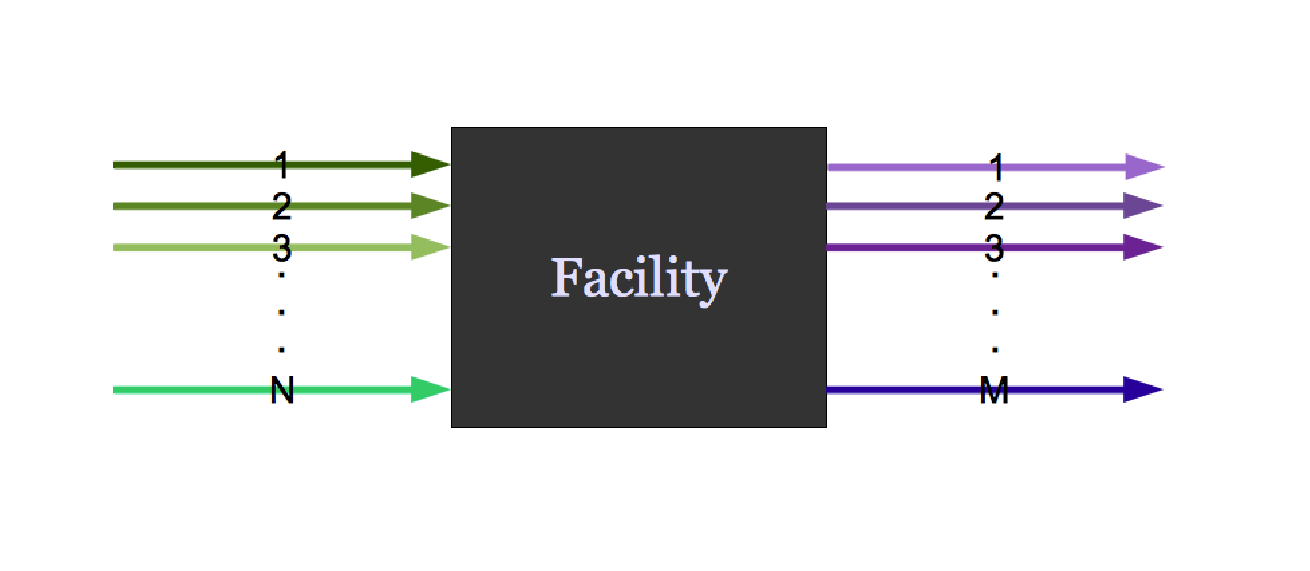
\includegraphics[height=4cm]{./images/facs.eps}
    \caption{Facilities as black boxes. \cite{cyclus2012}}
    \label{fig:facs}  
  \end{figure}

\end{frame}

\begin{frame}[ctb!]
  \frametitle{Motivating Question}
  
  \begin{block}{Dynamic Resource Exchange}
    If facilities are treated as individual black boxes and connections between
    facilities are determined dynamically, how does one match suppliers with
    demanders considering supply constraints and, supply response to
    quality-based demands, and issues of fungibility?
  \end{block}

\end{frame}
